\chapter{VR Interface}

In this chapter, I'll go into the implementation details of the VR interface. 
The requirements for the interface are as follows:
\begin{enumerate}
    \item It needs to report the 6-DOF poses of left and right hands as well as additional buttons for locomotion and gripper control. 
    \item Stereoscopic images need to be streamed and displayed on the VR headset to create depth perception for the wearer. 
    \item It needs to connect to both the simulation codebase written in Python and the real-robot controller written in C++. 
    \item The latency should be low and the computation speed should be fast so that the wearer can provide demonstrations with ease. The computation resource consumption should be low because the simulation and whole-body controller are resource-intensive.
\end{enumerate}

First, an overview of the architecture is given. Then, I justify some of the design decisions. Finally, I analyze the performance of the system.

\section{Architecture}

\begin{figure}
	\centering
	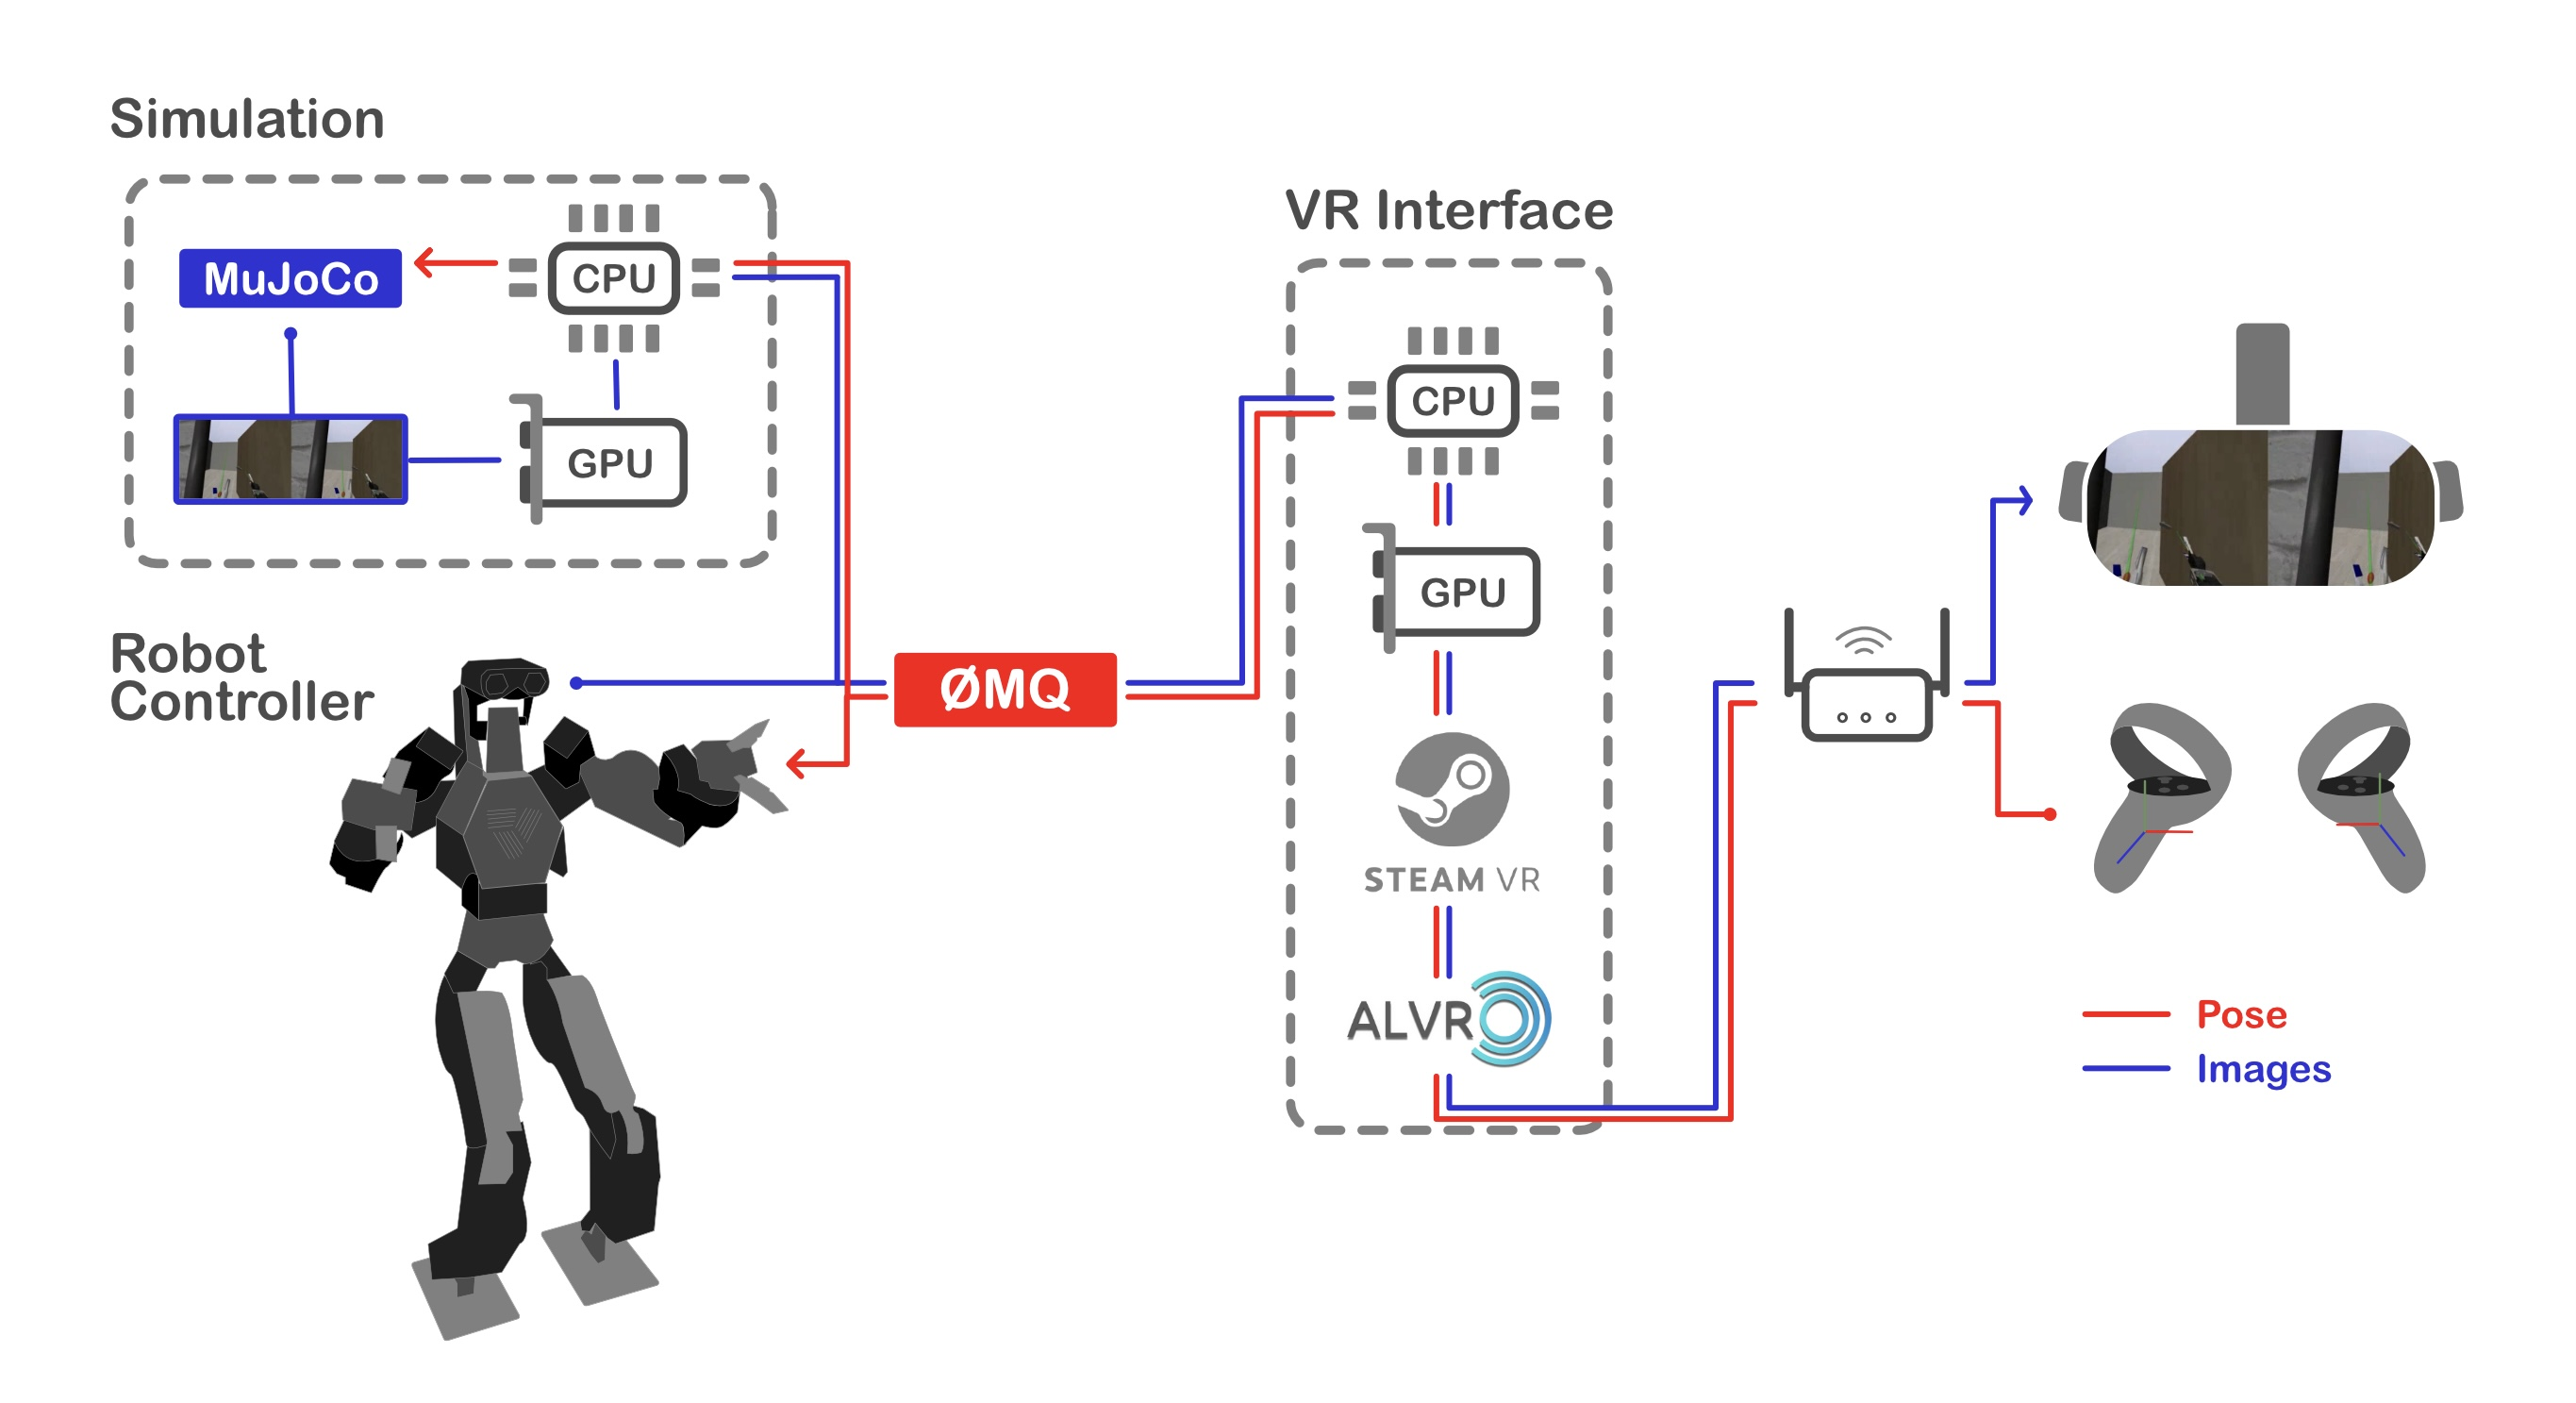
\includegraphics[width=\linewidth]{architecture_diagram.jpeg}
	\caption{Architecture for the VR interface}
    \label{fig:vr-interface}
\end{figure}

Figure \ref{fig:vr-interface} describes the software architecture. The VR interface code written in C++ runs on a separate laptop, which is connected to either the simulation desktop or the robot control station for the real robot. We use OpenVR (implemented in SteamVR) and ALVR (Air Light VR) for the communication between the laptop and the headset. OpenVR is a low-level API for VR applications designed to support a wide range of VR devices. ALVR is an open-source project that allows streaming Steam VR games from the laptop to the headset via Wi-Fi. It implements technologies such as Asynchronous Timewarp and Fixed Foveated Rendering for a smoother experience. ZMQ is an asynchronous messaging library that simplies message-passing between different programs or devices. 

For the simulation, we use Mujoco with Python binding for the physical simulation and Robosuite for the objects in the scene. We first render the scene using a virtual stereoscopic camera that is adjusted to match the interpupillary distance of the VR headset. Then, the rendered pixels are copied from the GPU to CPU and sent to the VR interface using ZMQ and ethernet. The interface code listens to the images and writes them into a GPU texture used by OpenVR. Finally, SteamVR and ALVR transmits the images through a router and displays them in the VR headset. At the same time, the interface polls the VR headset for the poses of the headset and controllers through OpenVR. It transforms the controller poses to the local frame of the headset, and they are then mapped to the poses of the robot hands in the robot's local frame. The latter mapping involves aligning the rotation axes of the controller with the axes used in the simulation. Let $R_t$ be the transformation between the VR axes and the simulation axes, $R_{vr}$ be rotation of the controller from its natural orientation, and $R_{sim}$ be the desired rotation to be applied to the robot hands. Their relation can be expressed as 
$$
R_{sim} = R_t^{-1} R_{vr} R_t
$$
The transformed hand poses are then published continuously using a ZMQ pub socket. When the simulation needs a VR command, it pulls the most recent command from the queue and sends it to the whole-body controller. 

The setup for the real robot is similar. However, since the robot has a lot more components to manage, I'll describe it in more details in the next chapter.

\section{Design Choices}

\subsection{OpenVR}

Initially, I created a website based on WebXR and JavaScript to stream controller poses over the internet. I wanted to improve the latency by keeping the connection within a local network, but I needed to set up HTTPS certificates in the campus lab, which was difficult. After getting tired of tunneling my connection over the internet, I decided to pursue a more low-level approach. 
I could use the native Oculus SDK, but this would limit the option to change VR systems in the future. Unity is a good option for cross-platform compatibility, but since I only need to stream images and controller poses, it is an overkill. I also don't think Unity exposes the low-level functionality to directly show the stereoscopic images. Since Unity uses the low-level OpenVR API, I decided to use it directly. Although a newer API called OpenXR is gaining steam, I feel that the performance benefits of OpenXR doesn't justify its complexity compared to OpenVR. 

Using OpenVR has several advantages. First, it has great performance since video games depend on it, which means that it has direct support from VR headset manufacturers. Second, it delegates the work of video streaming to SteamVR-compatible software such as ALVR. Third, it works on a variety of Operating Systems and targets many VR headsets. In comparison to \cite{arunachalam2022holodex} 

\subsection{Asynchronous Message Passing}
